A concurrent program has an acyclic communication topology if the underlying  communication graph undirected graph with threads as vertices and whose edges represent interactions between threads is acyclic. Then,   in our setting, atmost two threads of a program can access a variable. Thus such topologies can be viewed as a special case of $\twowriter$-systems. Acyclic  topologies have been previously studied by Chalupa et al. \cite{Data-centricDPOR}.  They show that acyclic topologies admits a polynomial time solution for the VSC-problem when a reads-mapping is given. 
But how do the complexity change when reads-mapping is not given? This is not yet known and we keep it as an open direction in this thesis. But after  invstigating VSC$^\pp$  for acyclic architecture we could successfully give a polynomial time algorithm. Looking at the result from a different perspective, we get a restriction on $\twowriter$ that yeilds a polynomial time algorithm for VSC$^\pp$.

\begin{theorem} \label{th:scacyclic}
\vscp  admits a polynomial-time solution  when the program architecture is acyclic.  
\end{theorem}

The above theorem will be proved in the next section.

\section{Algorithm}

We are given a program $\program$ with $k$ threads having a total of $n$ events across all threads, 
and a constant $\pp \geq 0$. The program $\program$ has an acyclic communication graph $\mathcal{G}$.

The Algorithm will be divided into two parts as in Section~\ref{VSCp} for $\onewriter$. Fix a program $\program$ with $k$ threads having a total of $n$ events across all threads, 
and a constant $\pp \geq 0$. Here is  overview of our algorithm. 
\begin{description}
\item[Step 1.] Guess a set $\points$ of at most $\pi$ events.
\item[Step 2.] Decide whether there exists an SC interleaving of $\program$ where the preemptions occur exactly after the events in $\points$.
\end{description}
As in Section~\ref{VSCp}, Step 1 can be done in $\mathcal{O}(n^{\pp})$. We select a set of $\pp$ preemption points from a set of $n$ events. 

\textcolor{red}{
For Step 2, we present an algorithm that has complexity $\mathcal{O}(n^3 \cdot k^2 \cdot \pp \cdot \pp!)$.  Hence, the overall complexity  comes to $\mathcal{O}(n^{\pp + 3} \cdot k^2 \cdot \pp \cdot \pp!)$.} Since $\pi$ is fixed, we get a polynomial-time algorithm for the \vscp\ problem for Acyclic programs. Step 2  can be further divided into four steps as shown in Figure~\ref{fig:schema-acyclic}. The first two steps is similar to Step 2.1 and Step 2.3 of $\onewriter$ and we do not describe it here again.

\begin{figure}[t]
\centering
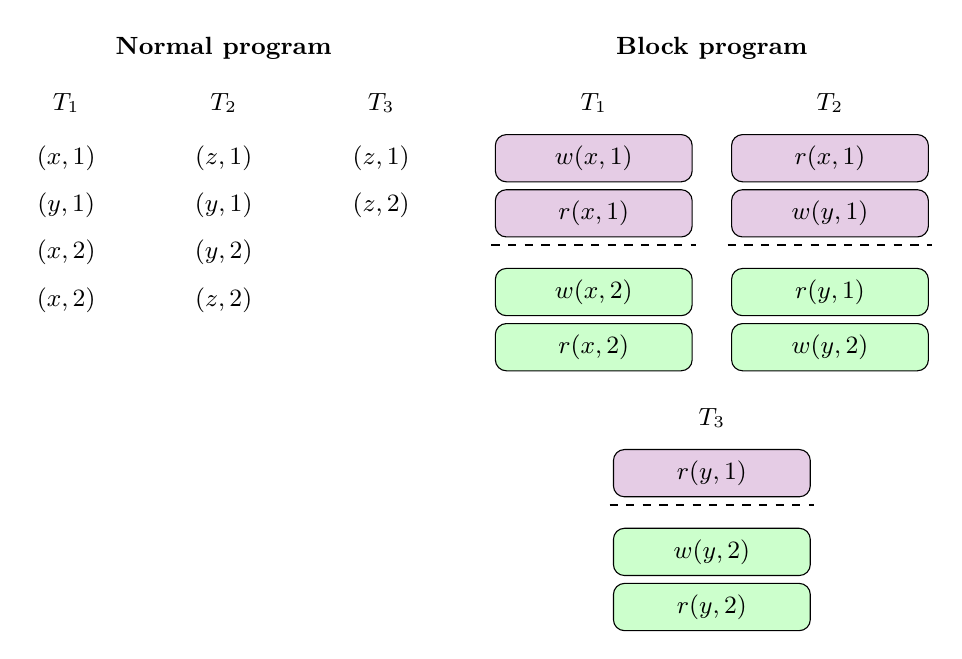
\begin{tikzpicture}[
    every node/.style={font=\small},
    innerblock/.style={
        draw,
        rounded corners,
        fill=violet!20,
        minimum width=2.5cm,
        minimum height=0.6cm,
        align=center
    },
    outerblock/.style={
        draw,
        rounded corners,
        fill=green!20,
        minimum width=2.5cm,
        minimum height=0.6cm,
        align=center
    },
    preemption/.style={
        dashed,
        thick
    }
]

% =========================================================
% NORMAL PROGRAM
% =========================================================

\node at (3.8,0.7) {\textbf{Normal program}};

% Three thread columns
\node at (1.8,0.0) {$T_1$};
\node at (3.8,0.0) {$T_2$};
\node at (5.8,0.0) {$T_3$};

% T1 events
\node at (1.8,-0.7) {$\wt(x,1)$};
\node at (1.8,-1.3) {$\rd(y,1)$};
\node at (1.8,-1.9) {$\rd(x,2)$};
\node at (1.8,-2.5) {$\wt(x,2)$};

% T2 events
\node at (3.8,-0.7) {$\wt(z,1)$};
\node at (3.8,-1.3) {$\wt(y,1)$};
\node at (3.8,-1.9) {$\wt(y,2)$};
\node at (3.8,-2.5) {$\rd(z,2)$};

% T3 events
\node at (5.8,-0.7) {$\rd(z,1)$};
\node at (5.8,-1.3) {$\rd(z,2)$};
%\node at (5.8,-1.9) {$\rd(,2)$};


% =========================================================
% BLOCK PROGRAM
% =========================================================

\node at (10.0,0.7) {\textbf{Block program}};

% ---------------------------------------------------------
% T1
% ---------------------------------------------------------

\node at (8.5,0.0) {$T_1$};

\node[innerblock] at (8.5,-0.7)
    {$w(x,1)$};

\node[innerblock] at (8.5,-1.4)
    {$r(x,1)$};

% Preemption point
\draw[preemption] (7.2,-1.8) -- (9.8,-1.8);

\node[outerblock] at (8.5,-2.4)
    {$w(x,2)$};

\node[outerblock] at (8.5,-3.1)
    {$r(x,2)$};


% ---------------------------------------------------------
% T2
% ---------------------------------------------------------

\node at (11.5,0.0) {$T_2$};

\node[innerblock] at (11.5,-0.7)
    {$r(x,1)$};

\node[innerblock] at (11.5,-1.4)
    {$w(y,1)$};

% Preemption point
\draw[preemption] (10.2,-1.8) -- (12.8,-1.8);

\node[outerblock] at (11.5,-2.4)
    {$r(y,1)$};

\node[outerblock] at (11.5,-3.1)
    {$w(y,2)$};


% ---------------------------------------------------------
% T3 -- below T1 and T2
% ---------------------------------------------------------

\node at (10.0,-4.0) {$T_3$};

\node[innerblock] at (10.0,-4.7)
    {$r(y,1)$};

% Preemption point
\draw[preemption] (8.7,-5.1) -- (11.3,-5.1);

\node[outerblock] at (10.0,-5.7)
    {$w(y,2)$};

\node[outerblock] at (10.0,-6.4)
    {$r(y,2)$};

\end{tikzpicture}
\caption{A concurrent program and its corresponding block-program representation.}
\label{fig:acyclic-block-program}
\end{figure}

\begin{itemize}
 \item[Step 2.1] \emph{Creating a block program based on $\points$}: Say thread $t_i$ of $\program$ has $\pp_i$ preemption points. Then there will be atmost $\pp_i+1$ blocks in $t_i$ with $\pp_i$ inner blocks.
 
 \item[Step 2.2] \emph{Choosing a permutation of the inner blocks}: We select a permutation among $\pp!$ permutations of the blocks. 
\end{itemize}

 Please refer to Section~\ref{VSCp} to recall the steps. At the end of Step 2.2, we have a block program based on $\points$ with distingusihed inner and outer blocks. We  along with a chosen permutation for inner blocks. 

 \begin{figure*}[t]
 \centering
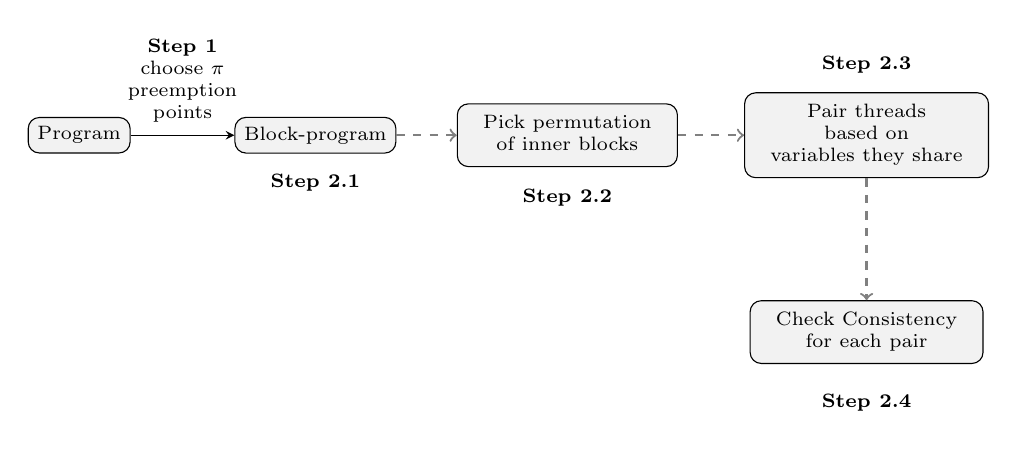
\begin{tikzpicture}[box/.style={rectangle, rounded corners, fill=gray!10, draw}]
  \node [box]  (a) at (0,0) {\scriptsize Program};
  \node [box] (b) at (3,0) {\scriptsize Block-program};
  \node [box] (c) at (6.2,0) {\scriptsize \begin{tabular}{c} Pick permutation \\ of inner blocks \end{tabular}};
  
  \node [box] (d) at (10,0) {\scriptsize \begin{tabular}{c} Pair threads\\ based on\\ variables they share \end{tabular}};
  
  \node [box] (e) at (10,-2.5) {\scriptsize \begin{tabular}{c} Check Consistency\\ for each pair \end{tabular}};
 
  

  \begin{scope}[->]
   \draw [>=stealth] (a) to node [above] {\scriptsize \begin{tabular}{c} \textbf{Step 1} \\ choose $\pi$ \\  preemption  \\ points \end{tabular}} (b);
   
   \draw [thick, dashed, gray] (b) to (c);
   \draw [thick, dashed, gray] (c) to (d);
   \draw [thick, dashed, gray] (d) to (e);
  \end{scope}

  \node at (3, -0.6) {\scriptsize \textbf{Step 2.1}};
  \node at (6.2, -0.8) {\scriptsize \textbf{Step 2.2}};
  \node at (10, .9) {\scriptsize \textbf{Step 2.3}};
  \node at (10, -3.4) {\scriptsize \textbf{Step 2.4}};
\end{tikzpicture}
\caption{Schema for the algorithm for Acyclic  programs}
\label{fig:schema-acyclic}
 \end{figure*}
 
\section*{Step 2.3. Pair threads based on common shared variables}

We denote $\varset_{i}$ as the set of variables accessed by thread $\thread_i$. 
For each pair of threads $\thread_i,\, \thread_j \in \program$ that have an edge in the communication graph $\mathcal{G}$,  calculate $X_{ij}=\varset_i \cap \varset_j$. As because we are dealing with a program with acyclic communication graph, we have: for all $i, \, i' \,j, \,j' \in \{1,2,\dots,k\}$ such that $i \neq i'$ or $\j \neq j'$, $X_{ij} \cap X_{i'j'}=\Phi$. 

Define $\bar{\threadset}^{\prog}=\{ \{t_i, t_j\}\mid X_{ij} \neq \Phi \}$ that contains all pairs of threads that communicate between them (access the same shared variable) in $\program$. Then size of $\bar{\threadset}^{\program}$ is $k-1$ as else the communication graph $\mathcal{G}$ would contain a cycle. We will omit any  superscript $\program$, whenever it is clear from context, for convenience. 

Each pair of threads in $\bar{\threadset}$ has already been divided into inner and outer blocks based on chosen set of preemption points $\points$. Moreover we also have selected a permutation on the inner blocks of the block program of $\program$. 

Next we pick an element from $\bar{\threadset}$, say $\{t_i$, $t_j\}$ and restrict the chosen  permutation of the inner blocks of $\program$ to the inner  blocks of these two threads. We call this restricted permutation $p_{ij}$.


We then insert the two outer blocks of $t_i$ and $t_j$ in $p_{ij}$ such that the resulting permutation is $\scmm$. 

We do the same for all $k-1$ elements of $\bar{\threadset}$.

\section*{Step 2.4. Check Consistency for each chosen pairs}

Threads $\{t_i,t_j\} \in \bar{\threadset}$ jointly have  $c_i+c_j$ inner blocks. We want to check if the outer blocks can be placed among the $c_i+c_j$ inner blocks in $p_{ij}$ so that the resulting interleaving of $t_i$ and $t_j$ is $\scmm$. This means that the resulting interleaving when restricted to $X_{ij}$, the set of shared variables accessed by $t_i$ and $t_j$ is $\scmm$. We do not explicitly use the term `restricted to $X_{ij}$' everytime we talk about interleaving of a subset of threads, however the intended restriction will be clear from the context.
%Say the last inner block of a thread $t_i$ is $b^e_i$. 
%Then the outer block of $t_i$ has to be placed after $b^e_i$ in any permutation including $p_{ij}$. 
Let $\bar{P}_{ij}$ contain all possible ways in which the outer blocks of $t_i$ and $t_j$ can be placed in $p_{ij}$. Size of $\bar{P}_{ij}$ is atmost $(c_i+c_j)^2$. For each element in $\bar{P}_{ij}$, we now check if it is sequentially consistent. If there exists one, we can conclude that for the chosen set of preemption points $\points$, there exists an $\scmm$-interleaving for $\program$. 

\paragraph*{Complexity} 

\smallskip

The proof of the algorithm follows from the following  lemma.

\begin{lemma}
Let $\program$ be a program with acyclic architecture. If there exists an $\scmm$ interleaving for each communicating pair of threads in $\program$, there exists an $\scmm$ interleaving for all the threads in $\program$. 
\end{lemma}
\begin{proof}
 Let $\{t_i,t_j\},\,\{t_u,t_v\} \in \bar{\threadset}^{\program}$ such that $i \neq u$ or $j \neq v$. Each pair  individually has an interleaving that is sequentially consistent when restricted to the shared variables accessed by them. 
 Order among events between any two threads is determined by the order in which their reads and writes access the common variable. Thus if the two threads $t_i,\, t_j$ do not have any variables in common nor is connected by a path in the communication graph $\mathcal{G}$, the order of their blocks will always satisfy $\scmm$ as long as the  program order is respected. 
 
 If there is a simple path in $\mathcal{G}$ like $t_i= t_{n_1}- t_{n_2}- \dots - t_{n_l}=t_j$, then $X_{n_u n_v}=\Phi$ if $v\neq u+1$ and $u \geq 1$, or else there will be a cycle in $G$. We can inductively show that merging all sequentially consistent interleavings from consecutive pairs in $t_i= t_{n_1}- t_{n_2}- \dots - t_{n_l}=t_j$, maintaining order between events in individual interleavings, does not violate $\scmm$. 
 
 
 Take a sequentially consistent interleaving $\sigma_{i}{i+1}$, $\sigma'_{i+1}{i+2}$ of threads $t_i$, $t_{i+1}$ and $t_{i+1}$, $t_{i+2}$ respectively. They can be merged into a single sequence $\sigma_m$ maintaining  the corresponding order of events in $\sigma_{i}{i+1}$ and $\sigma_{i+1}{i+2}$. This is because $t_i$ and $t_{i+2}$ have no events in common. 
 
% Draw two graphs $G^{\sigma},\, G^{\sigma'}$ corresponding to the two interleavings $\sigma$ and $\sigma'$ with the events of the interleavings as vertices. Draw an edge from vertex $u$ to vertex $v$ 
 
  We can show that even after merging  $\sigma_{{i},{i+1}}$ and $\sigma'_{{i+1},{i+2}}$ as a single sequence,  sequential consistentcy is not violated.  
  
If $e$ appears before $e'$ in $\sigma_{{i},{i+1}}$ or $\sigma_{{i+1},{i+2}}$ then $e$ appears before $e'$ even in $\sigma_m$. So program order is always satisfied in $\sigma_m$.  

Take any read $\rd(x,v)$ in the merged sequence $\sigma_m$. Then there must be a write in $\wt(x,v)$ before $\rd(x,v)$ in $\sigma_m$, with no other writes on $x$ in between. If $\wt$ and $\rd$ belong to the same thread, $\wt$ appears before $\rd$ in any interleaving which satisfies $\scmm$. If they belong to different threads, they must come from the pair $\{t_i,\, t_{i+1}\}$ or $\{t_{i+1},\, t_{i+2}\}$ and not both. WLOG if they belong to $\{t_i,\, t_{i+1}\}$, $\wt$ appears before $\rd$ in $\sigma_{{i},{i+1}}$ with no other writes on $x$ in between. Otherwise as only the pair $\{t_i,\, t_{i+1}\}$ has access to $x$, $\sigma_{{i},{i+1}}$ would not have satisfied $\scmm$. Again note that the events of $\{t_i,\, t_{i+1}\}$ has the same order in $\sigma_{{i},{i+1}}$ as in $\sigma_m$. Thus the conditions for $\scmm$ is satisfied by $\sigma_m$. 

Inductively, assuming the merged sequence $\sigma_{{i},{i+1}},\, \sigma_{{i+1},{i+2}},\, \dots,\, \sigma_{{j-2},{j-1}},$ satisfies $\scmm$, We can then show that $\scmm$ continues to hold after merging $\sigma_{{j-1},{j}}$. Since $t_{j}$ has no shared variables with $t_i,\, t_{i+1},\,\dots,\, t_{j-2}$, the same reasoning as before applies to prove $\scmm$.

\end{proof}
\smallskip

The above lemma is not depended on the block program or the choice of preemption points. It just states that acyclicity gives an advantage over the complexity of consistentcy checking as we just need to  consider if each pair of communicating threads are sequentially consistent.

Step 2.4 of the algorithm that we discussed  already gives a sequentially consistent interleaving for individual pairs in $\bar{\threadset}$. Hence the overall complexity is 







